\chapter{Implementation}
\label{chap:implementation}

\begin{figure}[H]
	\centering
	\label{fig:block}
	\includegraphics[width=0.7\textwidth]{../block/block.png}
	\caption{More technical blockdiagram of the Swakeup.}
\end{figure}

After the design choices had been made the blocks chosen had to be assembled. In fig. \ref{fig:block} the actual system architecture from a more technical
point of view is displayed. One can clearly see, that the system is divided into two physical boards. The logic board consists of the microcontroller, a serial
connection infrastructure, an OLED screen, an \textit{IEEE 802.11} module, a ISP
programming infrastructure and some LEDs/a button (UI).
\newpar  
The power board takes the 20 V input of a low-cost power supply and breaks it
down to 2.8 V (Vcc), 5 V for phone charging and the power which is needed for
the RGB LED.
\newpar
The partitioning of the system functionalities on two boards has a bunch of
advatages: Two people worked on this project, so each could develop a PCB; It is
quite common to seperate signals from power lines out of EMI reasons; There was
simply not enough space on one two-layer board for the whole system keeping a
base area of 5 cm x 4 cm, which was a design requirement. 
\newpar
The two boards are connected together through four headers. By these headers an
electrical and mechanical connection is maintained. The headers allow a feedback
from the LED driver on the power board to the logic board (ADC). Also the
control variable (PWM) comes via the headers from the µC to the LED driver. The
2.8 V Vcc is produced and regulated on the power board and is also availabe at
one header. Another voltage available from one header is the OLED driver
voltage. 

\section{Hardware}
\label{sec:hardware}
This section describes the two PCBs. Schematics can be found under appendix
\ref{append:power} resp. appendix \ref{append:logic}.

\subsection{Power Board}
\label{subsec:power}
It is the LM2840 which in combination with a simple voltage divider ensures the
2.8 V for Vcc. All step-down converters use the same inductor with a value of 33
µH. It is a low-cost, quite small, shielded inductor which is ment to be used
for switching power supplies. Moreover all step-down converters are enhanced
with a SMD schottky diode and of course at least one SMD capacitor for
smoothing the output signal. As it is good practice to do so all ICs are making
use of decoupling capacitors.  
\newpar
For charging ones phone the TS30012, another step-down converter IC, is used.
The feedback voltage divider of this IC is already integrated and does not need
to be provided externally as the IC provides fixed 5 V output. The output is
connected to a USB connector type A. This IC can deliver up to 2 A. An
interesting feature of the phone charging circuitry on the power board is the
"Dedicated Charging Port" (DCP) functionality. The TPS2514 is a small,
easy-to-use, 6-pin component, which complies to the USB standard and a majority
of the minefield of propriatary standards to signal a DCP. Now one might ask:
What does this mean? Well this means, that if you connect your IPhone, it will
know, that it can draw more than 100 mA, which is the minimum current provided
by a normal USB 2.0 port. Otherwise the current drawn by the phone will be
limited. The charging functionality can be turned on and off via a GPIO pin. The
TS30012 comes in a QFN16 package (pad pitch of 0.5 mm) to save space.
\newpar
For testing purposes a lot of test points have been included into the design.
Futhermore there are LEDs for different voltages (e.g. Vcc).
\newpar
The LED driver consists of an actual power electronics part and a feedback part.
The main idea is, that the current driven through the three color channels of
the RGB LED (see fig. \ref{fig:led}) can be controlled by software (PID
controller). In the power electronics part there are three analog circuits. Each
circuit mainly consists of a p-channel MOSFET, which is switched by a NPN
bipolar transistor. This bipolar transistor gets its intput signal from the
µProcessor (PWM). By pulling the 20 V to GND the PMOS "sees" a negative
gate-to-source voltage and opens. The additional bipolar transistor ensures,
that the gate-source capacity is charged fastly as soon as the PWM NPN blocks.
In this case the base is pulled up via \SI{10}{\kilo\ohm} to 20 V and as long as
the collector (which has the same potential as the gate of the PMOS) does not
also have 20 V the NPN keeps pumping charges into the gate-source capacity. The
simple silicon diode ensures that the gate-charging NPN has no effect as soon as
the PWM NPN opens. The rest of the circuit is again a standard step-down
converter. At the output of every single color channel power circuit one can see
a shunt resistor of \SI{0.1}{\ohm}. This shunt resistor is combined with a
simple low-pass filter. The feedback signal is amplified by a differential
amplifier which comes after the filter. The signal is supposed to be between 0 V
and 1 V (if the internal reference voltage is used). By doing so one can use all
bits of the ADC and therefore supress quantization noise. 
\newpar
So as there are three color channels (red, green and blue) one needs three
operational amplifiers. Hence the LM324QT, which provides four operational
amplifiers, has been chosen. Of course the decision has been made to take QFN16
packaging once more to save even more space. An additional operational amplifier
was now ready to be used as a digital-analog converter to drive the OLED screen.
For this reason a low-pass filter is attached to the input of the fourth opamp.
Apart from that the opamp is configured just like a standard non-inverting
amplifier. By software the OLED screen brightness is steerable. The feedback
from the OLED is generated with a voltage divider. 
\newpar
Figure \ref{fig:led} shows the kind of LEDs, which can be driven by this LED
driver.
\begin{figure}
	\centering
	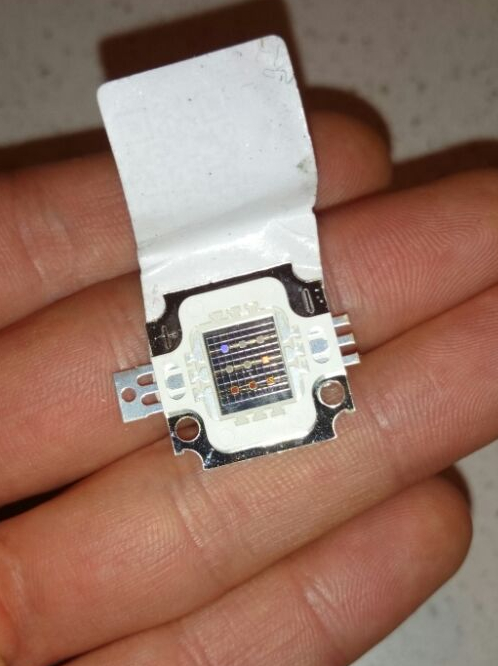
\includegraphics[width=0.3\textwidth]{./fig/led.jpg}
	\caption{10 W RGB LED}
	\label{fig:led}
\end{figure} 

\subsection{Logic Board}
The XMega will be programmed trough a PDI port. Furthermore four ADC and PWM pins are exposed for use with the power board. The screen is connected via a flat flex connector, rather than soldered directly on the board. This allows for reuse of the screen on further revisions without having to purchase new screens.\newpar
An external crystal is used for the real time clock. This gives the possibility to use the 32 bit real time counter on the XMega which is more precise than using a build in oscillator. Two low side n-channel MOSFETS are connected for reverse voltage protection. An external crystal for the system clock is also used, as the internal oscillator is not as precise, which increases serial communication errors.\newpar
The full schematics can be found in Appendix \ref{append:logic}.

\section{Software Interfaces}
As can be seen from the hardware, there are two systems that have to communicate with each other. Not only that, but its also needed to talk with a server back-end. The choice has been made to use Protobuf in order to save time. Protobuf, short for Protocol buffers, are a language-neutral, platform-neutral extensible mechanism for serializing structured data developed and maintained by google \cite{github:gpb}. This translates message structures in language dependent types. In C the messages are translated into structs, where the messages are translated into Objects in Java.
\section{Software Microcontroller}
\label{sec:software}
In order to facilitate all the functionality, code had to be written. Because the system is quite complex with many different functions, a good and clear structure has to be realized. Much of the development time has been invested in the writing and testing of underlying code which doesn’t have a direct result for the finalized product. In the following sub-chapters this system will be described, and explained why certain choices and compromises have been made.\\
In fig. \ref{fig:code_structure} below one approach of abstracting the code can be seen. Four layers are displayed with each dependencies on a lower layer. This has multiple advantages. Every block can now be swapped with different components while the system keeps running, if implemented well without breaches of layering.\newpar
For example, it's now possible to change microcontroller platform by only having to port the platform layer. Or if a different screen driver is used, only the software driver will have to be ported. Or of the application is meant to be changed, the application layer  has to be adjusted without any changes on the tightly integrated platform code. Other advantages are the reduction of having to test the whole system time after time, as it is possible to rely on the underlying layer if that is tested accordingly.\\

\begin{figure}[H]
	\centering
	\label{fig:code_structure}
	\includegraphics[width=0.6\textwidth]{../block/code_structure.png}
	\caption{The layered approach.}
\end{figure}
To make this layered code structure a reality, a small operating system has been developed which allows event driven communication, and a modular approach for driver and sub-systems. This modular approach also makes power saving easier as a module will be uninitialized when it's not used anymore. Removing any possibility for the developer of the system to forget to disable the peripheral/module.\newpar

\subsection{Operating System}
To make the previously discussed layering possible with communication, a small operating system has been developed with a minimum subset of functions. This subset is divided in two parts, Events and Modules.
\subsubsection{Module}
The modular system is realized by a struct. Every module contains a name, a usage counter, initialize and deinitialize functions, and dependencies. A module can be initialized by the "module\_init" function. This function will check for all the dependencies, whether they are already initialized. If this is not the case, it will be initialized including all the dependencies of the dependency. The "module\_init" function will also call the initialize function, which can be used for a module to set up registers for example. Once a module is not needed anymore, it can be de-initialized with the "module\_deinit" function. This function will decrease the usage counter for every dependency, and once a dependency is not used anymore it will also be de-initialized. This function also calls the de-initialize function of the given module.

\begin{minted}[baselinestretch=1, fontsize=\small, linenos,frame=single,framesep=5pt]{C}
#define MODULE_DEFINE(VAR, DESC, INIT, DEINIT, ...)     \
Module VAR = {                          	\
.init = INIT,                           \
.deinit = DEINIT,                       \
.cnt = 0,                               \
.name = DESC,                           \
.deps = { __VA_ARGS__ }                 \
} 
MODULE_DEFINE(CORE, "Central core", init, deinit, &TIME, &COMMAND, &ESP8266);
\end{minted}
In the code above a simplified usage example can be seen of this modular system

\subsubsection{Event}
For communication between modules an event based system has been realized. The developed system does not have any kind of priority for events, and events can be ignored if the event buffer is full because of a too heavy event. Every event contains a counter for debugging purposes, a pointer to data that can be given along with the event, and a description. An event can be created by use of the following code:
\begin{minted}[baselinestretch=1, fontsize=\small, linenos,frame=single,framesep=5pt]{C}
#define EVENT_REGISTER(eventName, desc)\
Event eventName = \
{.eventId = __COUNTER__, .data = 0, .description = desc, .descLen = sizeof(desc) }
EVENT_REGISTER(EVENT_UART_DELIMITER, "Got UART delimiter");
\end{minted}
Events alone do not serve any purpose without listeners. Thus it's possible to register listeners in the event system. With the "event\_addListener" function a module can listen to a certain event and provide a function to be called upon the reception of such an event. This can be seen in the code below:
\begin{minted}[baselinestretch=1, fontsize=\small, linenos,frame=single,framesep=5pt]{C}
event_addListener(&EVENT_UART_DELIMITER, callback);
\end{minted}
The listeners can be removed with the "event\_removeListener" function. The adding listeners is usually done in the initialization function, as the modules require these events during the period that they are active. In order to fire an event to all the listeners the following example can be used: 
\begin{minted}[baselinestretch=1, fontsize=\small, linenos,frame=single,framesep=5pt]{C}
event_fire(&EVENT_UART_DELIMITER, SYSTEM_ADDRESS_CAST (&delimiters[USART_ID][i]));
\end{minted}
This line of code will fire a EVENT\_UART\_DELIMITER event, and adds some information to go with it.\newpar
In order for these events to be processed the "event\_process" has to be called. This should be the only function called in the infinite while loop of the system. A way to save energy is to pass functions to the event system if the system is capable of a sleeping functionality. Now the system will sleep whenever there are no more events to process, or wake up when an interrupt occurs.

\subsection{Deriving functionality}
In fig.\ref{fig:block} the functions of the system can be observed, these functions can be translated into modules and a hierarchy can be created. Along with drivers for the hardware, some software drivers have been written as well. These software drivers provide support for internal development such as logging text in a proper fashion, and creating a way of executing commands on the device. All the platform drivers are interfaces to the system's peripheral. On top of this layer are the actual drivers. This houses the initialization code for the hardware drivers, and gives a way to access the functionality of the hardware without needing to know the registers/commands. The layer above this provides a more generic function set, where no knowledge of the hardware is needed anymore. This can then be used by the last layer, the Application layer. The application layer houses different applications, and a general state of the device can be found inside this layer.
\begin{figure}[H]
	\centering
	\label{fig:block_code}
	\includegraphics[width=0.5\textwidth]{fig/block_code.png}
	\caption{The system structure and hierarchy}
\end{figure}
Above in fig. \ref{fig:block_code} this translation from system design to a more refined code structure is shown. A brief description of the required functionality for every block follows. 

\subsection{Platform layer}

Every used peripheral has a platform driver. The UART driver has an input and output buffer, and is being used with interrupts. Two UART channels are being used, one for the ESP8266 and one for the USB-Serial converter. The SEP525F has a SPI interface without a need or possibility to read, the SPI driver contains only blocking write. This should be changed to DMA and interrupt transfers. The timer sets up the real time counter for the second pulses, and has functions to set the PWM of every channel for the power board. And lastly, the ADC peripheral. This scales the voltage read from the input pins and provides it to whoever needs the ADC values.
\subsubsection{UART}
The UART module delivers all the communication to the USB-Serial converter and ESP8266. The code has been kept as generic as possible so that adjustments to the external hardware has no influence to the driver code. It would even be possible to move to a different xmega model with more USART ports since a macro is used for generating the interrupt code. Every USART port has a status, an array with delimiters, an in and output buffer, a sending status and an id. The status contains variables for the buffers, and allows for a ring-buffer usage. A ringbuffer is chosen as it has little overhead compared to lists or queues, the order of the data matters, and we don't expect to go outside of our given buffer capacity. The delimiters are used for the USART to listen to certain characters on the receiving data. Once there is a match an event will be fired. The example below shows the usage of this delimiter.
\begin{minted}[baselinestretch=1, fontsize=\small, linenos,frame=single,framesep=5pt]{C}
uint8_t uart_add_delimiter(char delimiter, USART_t * port);
static void callback(Event * event, uint8_t * data) {
if(event == EVENT_UART_DELIMITER){
struct UartDelimiter * delimiter = (struct UartDelimiter*)data;
if (delimiter->port == &ESP_UART_PORT) {
//Read buffers etc
}
}
}
static uint8_t init(void) {
uart_add_delimiter('\n', &ESP_UART_PORT);
event_addListener(&EVENT_UART_DELIMITER, callback);
return 1;
}
\end{minted}
In this example, a certain module will tell the UART module to listen for a new line character, and the module will subscribe to the event. The UART module passes the delimiter information with it, so that there is knowledge about how much data can be read since the last delimiter event.\\ 
The interrupts are generated with the macros that can be found at appendix \ref{append:usartinterruptgen}.
The following code can be used to generate the interrupt code for every USART channel:
\begin{minted}[baselinestretch=1, breaklines=true, fontsize=\small, linenos=true,frame=single,framesep=5pt]{C}
USARTRXCISR(USARTE0, DEBUG_UART,     USARTE_ID, received);
USARTDREISR(USARTE0, DEBUG_UART,     USARTE_ID);
USARTRXCISR(USARTD1, ESP_UART_PORT,  USARTD_ID, );
USARTDREISR(USARTD1, ESP_UART_PORT,  USARTD_ID);
\end{minted}
Since the system could be writing to the buffer that is being handled in the interrupt, a lock has been implemented to prevent unexpected outcome. One lock waits while the lock signal is freed, while the other lock function returns a 0 upon failure to acquire the lock.
\begin{minted}[baselinestretch=1, fontsize=\small, linenos,frame=single,framesep=5pt]{C}
#define lock(id) while (outBufferLock[id]); outBufferLock[id] = 1
#define unlock(id) outBufferLock[id] = 0

static inline uint8_t softlock(uint8_t id) {
if (outBufferLock[id]) return 0;
outBufferLock[id] = 1;
return 1;
}
\end{minted}
The USART on both channels have the same settings: 8 bit words, medium level interrupts and a baudrate of 115200. This baudrate can go higher once the whole system is tested with good results.
\subsubsection{SPI}
The SPI driver is incomplete as is, a lot of performance optimizations can and should be done. One of the biggest disadvantages at the moment is that it is blocked writing. When a lot of data is being sent consecutively by the SPI driver, the event buffer fills up and might even get full. Interrupt based design should be looked at and investigated, as this would still allow the events to be handled. The caveat with this, however, is that a large buffer has to be allocated for the SPI. And memory is costly. DMA is another technique to solve the problem, this would eliminate the need for a CPU at all and give the system all the time to process the other tasks. One needs to be cautious, as DMA has overhead on low data amounts.
\subsubsection{Timer}
The Timer design is incomplete, and only houses a RTC. Due to a hardware failure, the internal crystal is being used. Which implies a worse accuracy than an external one. However since the most recent time can be retrieved from the internet this is not a major issue. Future additions to the Timer module include: Alarm function for timeouts on waiting, PWM functionality and using the 32 RTC with the external crystal. The Timer module is set up to use it's overflow interrupt. The period is set to 1023. As soon as the counter reaches 1024, a second pulse event will get fired and the run time will get incremented.

\subsection{Driver layer}
\subsubsection{SEPS525F}
As mentioned before, the screen uses a SEPS525F IC. This driver drives allows for driving screens with a resolution of up to 160x128 pixels with 18 bit combined color. This means that there are 6 bits for blue, 6 bits for green and 6 bits for red. However this would require to send 3 bytes for 2 bits of color precision. There is also a 16 bits combined color option available, which has been used in this driver. 5 bits for blue, 6 bits for green and 5 bits for red. A 24 bit color (8 bits per color, 0-255) can be converted with the following define:
\begin{minted}[baselinestretch=1, fontsize=\small, linenos,frame=single,framesep=5pt]{C}
#define SEPS525F_TO656(r,g,b)((r>>3)<<11)|((g>>2)<<5)|(b>>3)
\end{minted} 
The SEPS525F has three data interfaces that could be used: SPI,
RGB, Parallel. In retrospect a parallel interface would have given major
performance advantages. However due to time constraints a SPI interface has been
chosen. The clock frequency of the SPI is set at the CPU speed divided by two.
Which is a clock of 8 MHz when not in any power saving mode.\newpar The SEPS525F
has two modes, a data mode and a command mode. With the command mode a register
can be set. In order to achieve this the register will be written first, while
clearing the RS and the CS pin. Once the register is written, the RS pin will be
set while keeping the CS pin low. After the data is written the CS pin will be
set.  
\begin{minted}[baselinestretch=1, fontsize=\small,
	linenos,frame=single,framesep=5pt]{C}
static void SEPS525F_reg(int idx, int value) {
SEPS525F_PORT.OUTCLR = SEPS525F_CSB | SEPS525F_RS;
spi_write_blocked(idx);
SEPS525F_PORT.OUTSET = SEPS525F_RS;
SEPS525F_PORT.OUTCLR = SEPS525F_CSB;
spi_write_blocked(value);
SEPS525F_PORT.OUTSET = SEPS525F_CSB;
}
\end{minted}
This can be seen in the code above. The driver gives the possibility to draw a single pixel, but it's significantly faster to write multiple pixels at once. For this a region that will be drawn on has to be set. Then the driver ic will expect a certain amount of pixels, which have to be written as data. According to the datasheet special scrolling features should be available, however this is not explained later on in the datasheet. There are a lot of parameters that can be set for the screen, such as duty cycle, frame rate, driving currents. The explanation of all these can be found in the datasheet, just like the recommended values. The given initialization sequence of the datasheet did not work, so an Arduino library has been ported successfully\cite{github:oled}.
\subsubsection{Terminal}
The Terminal driver gives the possibility to format strings, and outputs the formatted strings to a sink. The default sink writes to the USB-Serial IC via the UART driver. Formatting is done via the tinyprintf library\cite{sparetimelabs:tinyprintf} and implements the 'd' 'u' 'c' 's' 'x' 'X' formats.
\subsubsection{ESP8266}
The ESP8266 is a low cost Wi-Fi module which can be flashed with own firmware. This firmware is written using Sming in C++, more on this in chapter \ref{sec:esp}. In order to establish communication, protocol buffers are used. The ESP8266 driver implements a stream that is used by the Control Module which will be explained in the next section. The XMega will also serve as a bridge to flash the firmware on the ESP8266, as the module has to be detached from the board to program it right now. 

\subsubsection{ADC}
The Xmega subsumes a quite powerful ADC. This ADC can be used with four
different channels. The SAR ADC almost feels like being four ADCs as one
conversion does not have to be completed befor anotherone starts. The single
bits are independent of each other (pipelining). The ADC driver is designed for
four different channels (red, green, blue, oled). It runs in single conversion
mode and a couple of conversions is triggered to fill a buffer to enable
averaging, which is recommended for such an application. The drivers is written
quite generic to not have to write the same code for each channel with other
register names. This can be seen e.g. in the following code example. 

\begin{minted}[baselinestretch=1, fontsize=\small,
	linenos,frame=single,framesep=5pt]{C}
/////////////////////////////////////////////////////////////////////////////////
// Macro: Create ISRs for the individual channels.
/////////////////////////////////////////////////////////////////////////////////
#define CREATE_ADCA_ISR(ADCVECTOR, VARSEMAPHORE, BUFFER, RESULTREG,STARTFLAG) \ 
ISR(ADCVECTOR) \ 
{ \ 
	static volatile uint8_t cycles = 0; \
	if(!VARSEMAPHORE) \ 
	{ \ 
		if( ((int16_t) RESULTREG) < 0) \
			BUFFER[cycles++] = 0; \ 
		else \ 
			BUFFER[cycles++] = RESULTREG; \ 
		if(cycles < NU_AVERAGING_VALS) \ 
		ADCA.CTRLA |= STARTFLAG; \ 
		else\ 
		{\ 
			VARSEMAPHORE= 1;\ 
			cycles = 0;\ 
		}\ 
	}\
}
\end{minted}

\subsection{PWM}
A special thing about the PWM hardware in the Xmega is, that two high-resolution
modes are available. This enables the possibility to make the PWM periphery
input frequency up to 8 times higher as the system clock. This nice feature
enables high PWM frequency, with still a quite accurate resolution of the duty
cycle. The PWM driver also is written generically for four different channels
(red, green, blue, oled).

\subsection{Module Layer}
Although all the drivers talked about before make use of the Module system, they are not located on the Module layer. This is a naming convention mistake.
\subsubsection{Command}
The Command module has the purpose of setting up an accessible possibility to execute commands received by the USB-Serial connection. It is possible to register up to 26 commands. One for every letter in the alphabet. A command can be registered by use of the following code:
\begin{minted}[baselinestretch=1, fontsize=\small, linenos,frame=single,framesep=5pt]{C}
command_hook_description(
'T', &terminalCommand, "Log sink    T<option> options: U(Uart) S(Screen)\0"
);
\end{minted}
It takes 3 arguments, the first one being the letter the command is tied to. The second one is a function pointer for the callback. And the third one is a usage description that can be requested by the user by writing a '?' to the terminal. In fig. \ref{fig:command_usage} an example output can be seen.
\begin{figure}[H]
	\centering
	\label{fig:command_usage}
	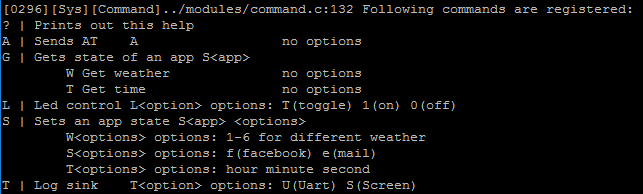
\includegraphics[width=1\textwidth]{./fig/command_usage.png}
	\caption{Response of a question mark}
\end{figure}
It's up to the developer to parse the string that is passed with the command. An example input string could be:"ST 12 23 34" which sets the time to 12:23:34. The callback will receive the same string as thats sent, minus the command character. Some helper functions have been written such as "command\_next\_int" to make parsing easier. Parsing the example string is done in the following code:
\begin{minted}[baselinestretch=1, fontsize=\small, linenos,frame=single,framesep=5pt]{C}
uint8_t index = 1;
if(data[index-1] == 'T'){
uint32_t hour = command_next_int(&index, data, len);
uint32_t minute = command_next_int(&index, data, len);
uint32_t second = command_next_int(&index, data, len);
}
\end{minted}
\subsubsection{Control}
The name for this module might be confusing, but it controls all the inter
system communications. The Control module defines streams and has the capability
to encode and decode Protocol buffers messages. At the moment of writing only
one stream is implemented, which is the ESP8266 stream. This is used to talk
with the ESP. Eventually all the communication to the PC should also happen via
a stream. There is a small protocol beneath the protocol buffers. Protocol
buffers itself does not offer a possibility to send and receive multiple
messages, so a length of the outgoing data has to be sent first. Other than the
length of the messages, the protocol also contains a prefix of 4 bytes, so that
the stream can get up to date again if there is some sort of data loss. Google
does not use a protocol buffers implementation for C, this is why NanoPB
https://github.com/nanopb/nanopb has been used as an external library. NanoPB
has a smaller code footprint, and has options to handle and print out error
messages.

\subsubsection{Light Controller}
The light controller is mainly a big state machine which accesses a queue. By
using the light controller module other code can post colors to the queue. It
can be specified which color the LED shall have for how long. There are two
different modes: The first mode is just playing the color ones and removes it.
The second mode repeats all colors in the given order once they are in the
queue. A special feature of the light controller is a interpolation algorithm to
allow three-dimensional fading between different colors within a given period.
Furthermore the relative brightness of a color can be regulated. The light
controller module makes use of the PID controller, to steer the lights. A
selfmade fixed point library is used for calculations.

\subsubsection{PID Infrastructure}
The PID module is one of the most basic modules. It is written in a handy way.
The module provides algorithms to realize PID controllers. Code, which utilizes
this modules, simply spawns a controller by using the
\myemph{add\_Controller(mycontroller\_t *newController)} function. That way a
controller e.g. simulated and developed with Matlab can easily be added to the
system. The e.g. setpoint can easily be manipulated by the owner of the
controller (i.e. some higher layer user). Via macros the debugging output can be
adjusted (save code size) and necessary output for PID controller tuning can be
optained. The PID arithmetics are executed with the help of the fixed point
library.
\begin{figure}[H]
	\centering
	\label{fig:pid}
	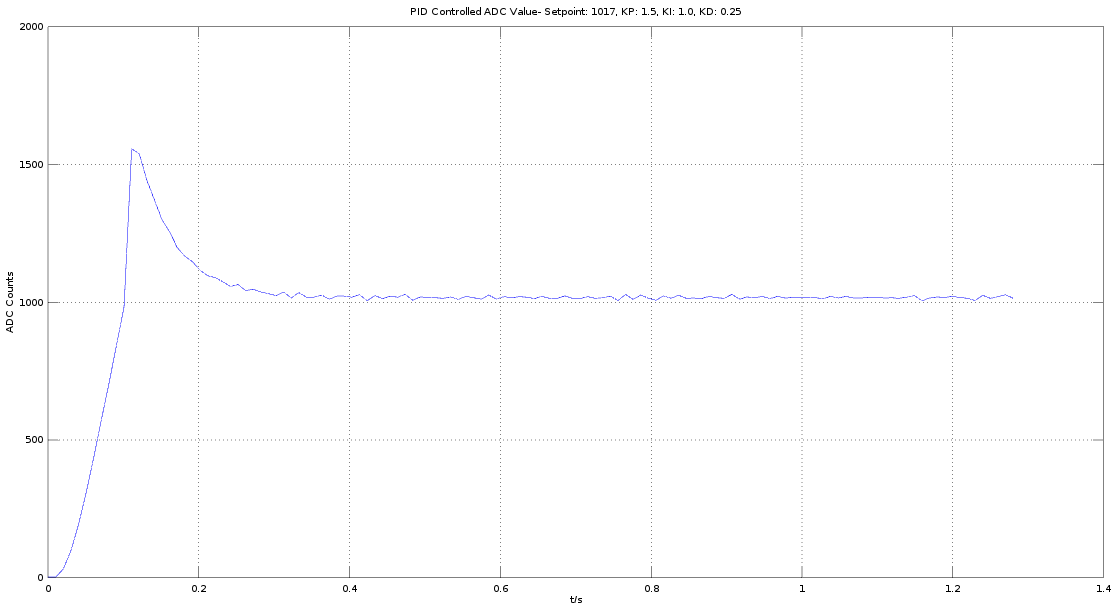
\includegraphics[width=1\textwidth]{./fig/pid_12v_100Hz.png}
	\caption{Step-response of a PID controller for the screen voltage
	control with 100 Hz periodicity.}.
\end{figure}

\subsubsection{Voltage Controller}
The voltage controller module makes use of the PID controller module by defining
a PID controller to controll the scrren voltage to a given setpoint. This setpoint is calculated using the self-made fixed point library, taking the voltage divider
and the reference voltage of the ADC into account.

\subsubsection{LOG}
Almost every  or module has a dependency on the LOG driver. In order to use the logging functionality, a file first has to initialize the logger. this is done by calling:
\begin{minted}[baselinestretch=1, fontsize=\small, linenos,frame=single,framesep=5pt]{C}
LOG_INIT("Core");
\end{minted}
This is required to keep track of where the logging happens. There are multiple levels of logging, which currently all have the same effect other than the name, except for the "LOG\_ERROR" function. The error log function halts the system. In a future build there should be a possibility to set a general log level so that log statements with less importance than the general log level will not be written. Every log is translated to the following three statements:
\begin{minted}[baselinestretch=1, fontsize=\small, linenos,frame=single,framesep=5pt]{C}
#define LOG_INTERNAL(LEVEL, MSG, ...) \
log_message("[%04d][%s][%s]%s:%d ",timer_runTime(),LEVEL,log_name,__FILE__,__LINE__);   \
log_message_p(PSTR(MSG), ##__VA_ARGS__);                                                        \
log_message("\r\n")
\end{minted}
An example like:
\begin{minted}[baselinestretch=1, fontsize=\small, linenos,frame=single,framesep=5pt]{C}
LOG_SYSTEM("Received command: %c", command);	//command is a character
\end{minted}
Produces the following string on the sink: "[2727][Sys][Command]../modules/command.c:157 Received command: T". The string contains the absolute runtime, what kind of log it was (debug, system, warning), the filename and the file line. The strings are saved in the flash to save memory. If the sink for the terminal changes, so does the output for the logger, as its depending on the terminal. The screen can be used to log to. This can be seen in fig. \ref{fig:screen_logger}.
\begin{figure}[H]
	\centering
	\label{fig:screen_logger}
	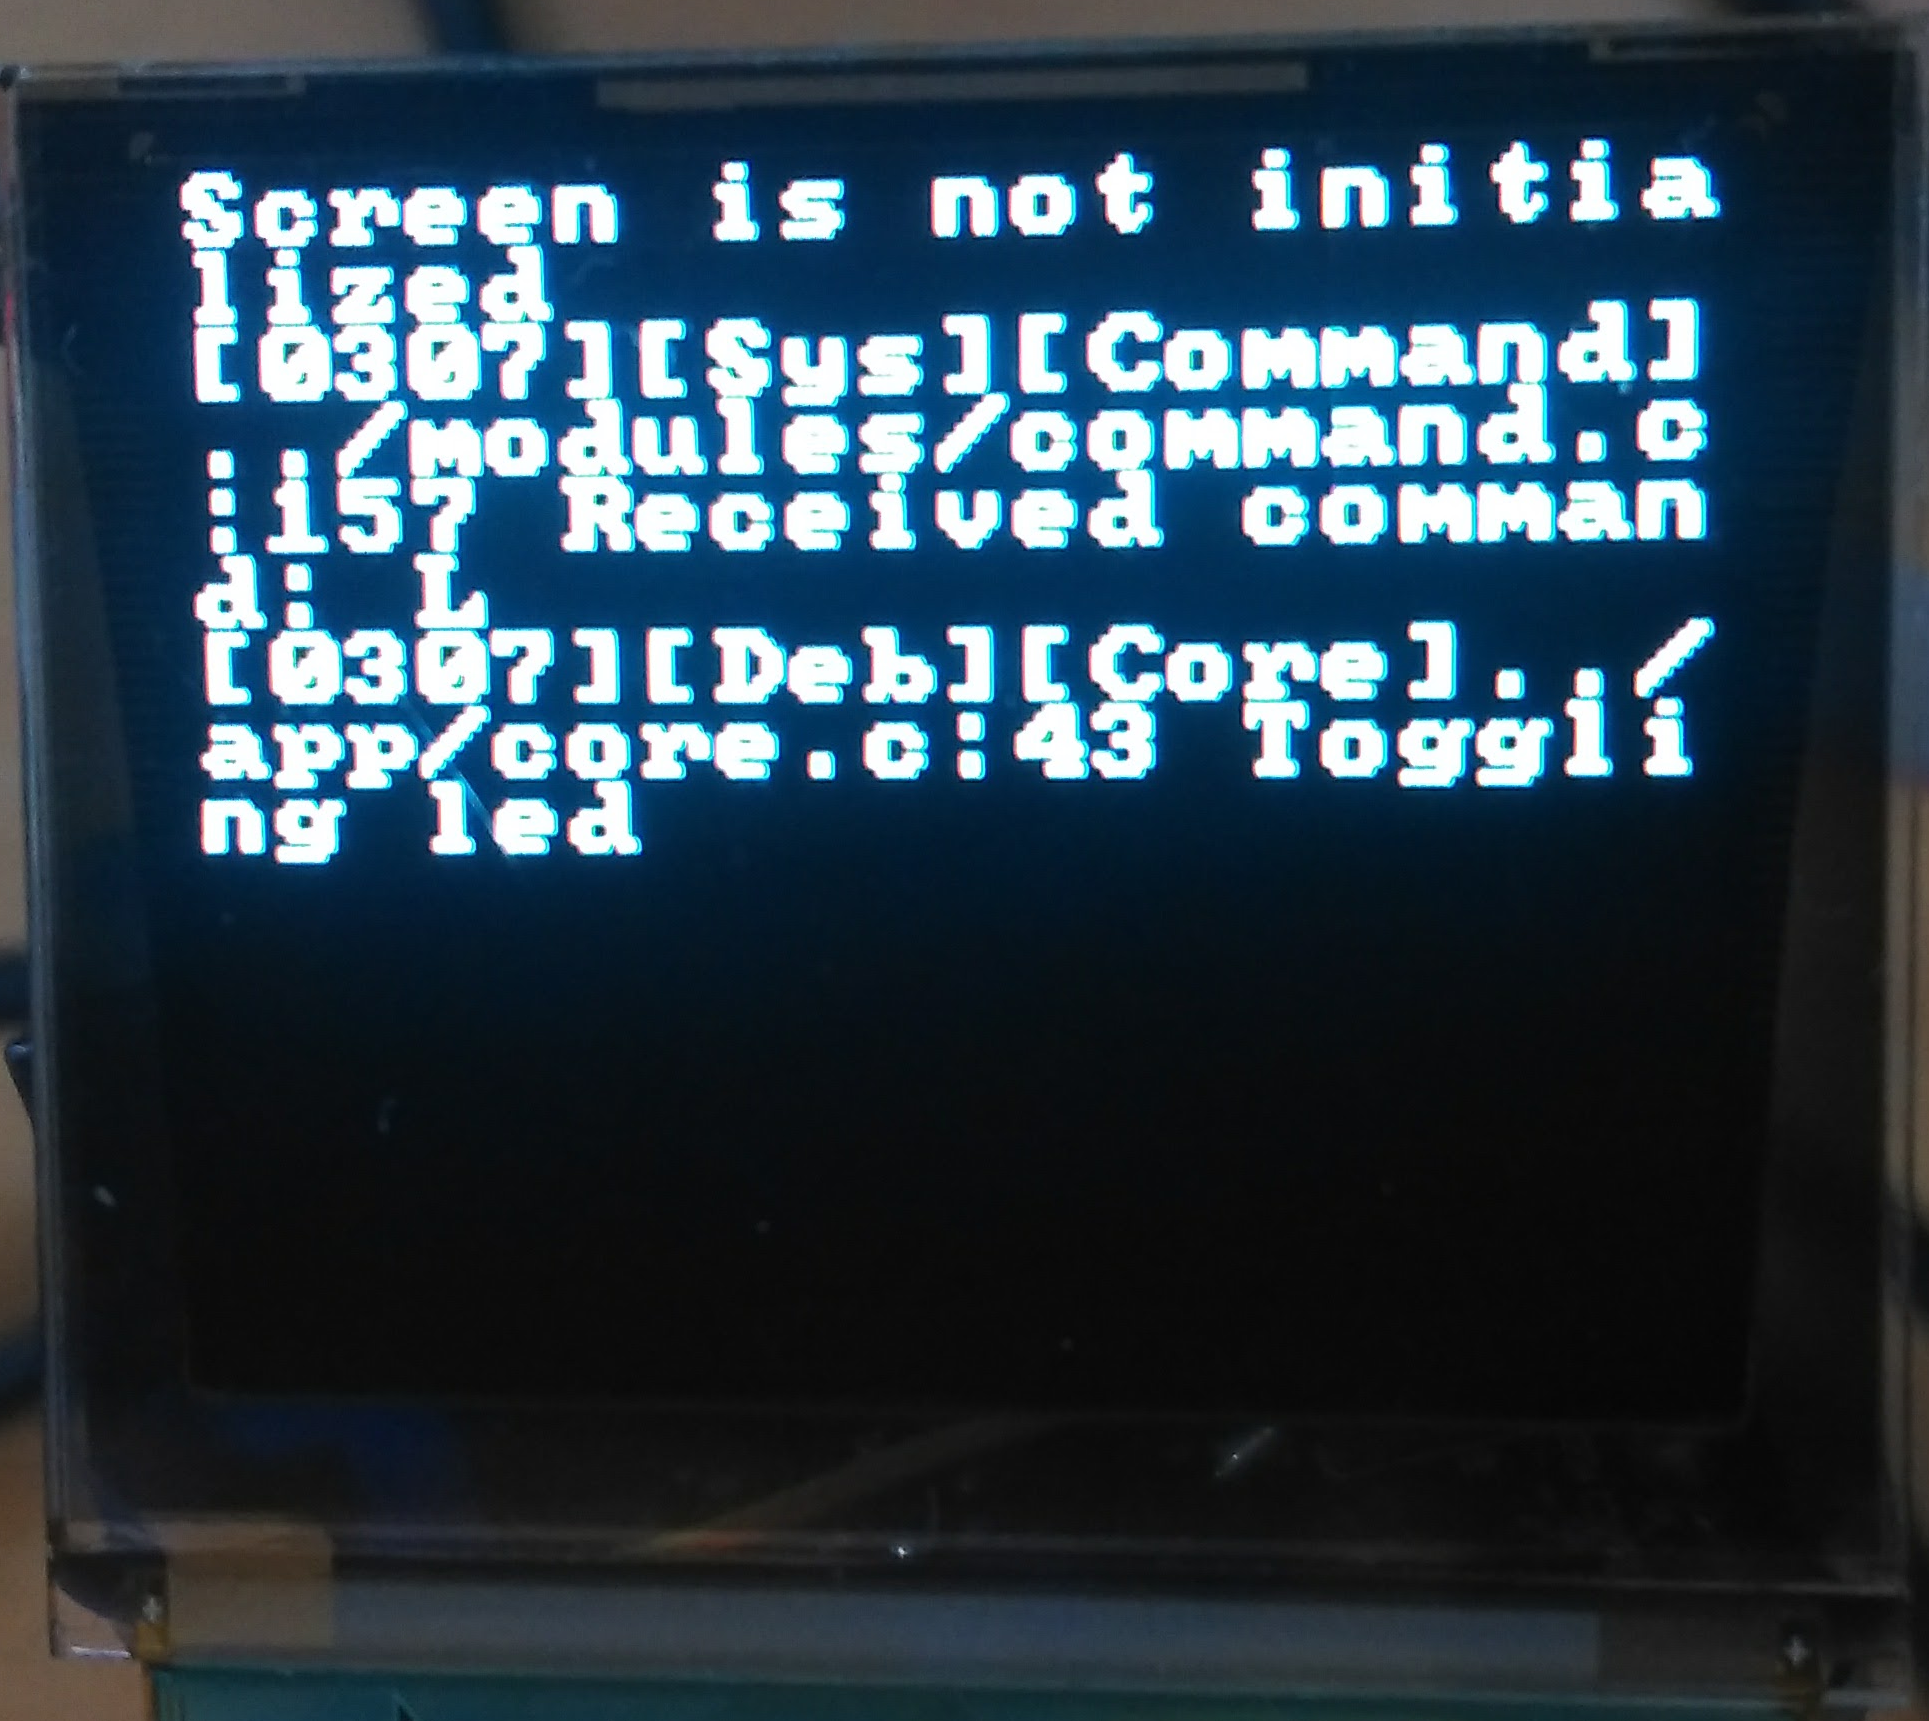
\includegraphics[width=0.4\textwidth]{./fig/screen_logger.png}
	\caption{Redirecting the output to the screen}
\end{figure}
However this has to be used carefully, as writing to screen takes significantly longer than outputting it over UART. So the system might freeze in case of too much text to show. If needed it's also possible to disable all the logging for certain log levels. This can be useful if there is no interest in debug messages from a module. This can be done by calling LOG\_LEVEL\_SET with the minimum wanted log level.
 Lastly there is a functionality to adjust the formatting of the log on the output. For logging on the screen it might not be desirable to show all file names and line numbers. This is done by calling the log\_set\_display function.
 \begin{minted}[baselinestretch=1, fontsize=\small, linenos,frame=single,framesep=5pt]{C}
 log_set_display(LEVEL_NAME); // Only show the level (debug, warning) and module name
 log_set_display(DEFAULT_LOG_FORMAT); // Returns to default formatting
 \end{minted}

\subsubsection{Screen}
The Screen module contains routines for drawing shapes, images and text on the screen. Currently implemented shapes include: Rectangle, filled rectangle, circle, filled circle, pixel, and line. These shapes are drawn with the color that is currently set. Images can be drawn both from flash and from memory. Better practice reads them out from flash, as there is little memory available. A start and stop function is available. This can be used to denote whether the shapes should be filled, or whether only the outline should be drawn. Another future addition can speed up the drawing significantly when a data start and data end command will be sent upon calling start and stop. This is not implemented in the current version.
\subsubsection{Time}
The Time keeps track of time offline. It does so by keeping track of hours minutes and seconds, and incrementing them accordingly upon every second pulse generated by the Timer driver. The time can also be set via a function.

\subsection{App layer}
This layer is the least elaborated, as it has the last priority since it would not work without the layers before it regardless.
\subsubsection{Clock}
The clock application draws a digital clock, alarm and date. It listens to time
updates, and updates the time unit that has been updated, whether that is second
minute hour or a combination of them. Moreover the clock app includes the alarm
functionality, which makes it possible to set an alarm and to react on it (play
a certain light pattern via the light controller). 
\subsubsection{Weather}
The weather application draws a temperature, unit and an icon based on the weather situation (rain, snow, sun, overcast) which are being drawn via screen routines. 
\subsubsection{Mail}
The mail application draws mail icons and shows the 4 most recent emails with the first 5 letters of the sender and first 5 letters of the subject.
\subsubsection{Status}
The status application draws the status bar. This reflects whether the alarm is set, whether the light is on and what the signal strength is
\subsubsection{Console}
The console application controls the screen terminal, in the future it will also be capable of receiving commands over WI-FI, however that functionality is not in yet due to time constraints.
\subsubsection{Core}
The Core translates all the commands given to actions, places graphical user interface elements on the screen, and has the possibility to enable and disable applications. Currently this results in fig. \ref{fig:clock_weather} below. All the applications have their own green bounding box space
\begin{figure}[H]
	\centering
	\label{fig:clock_weather}
	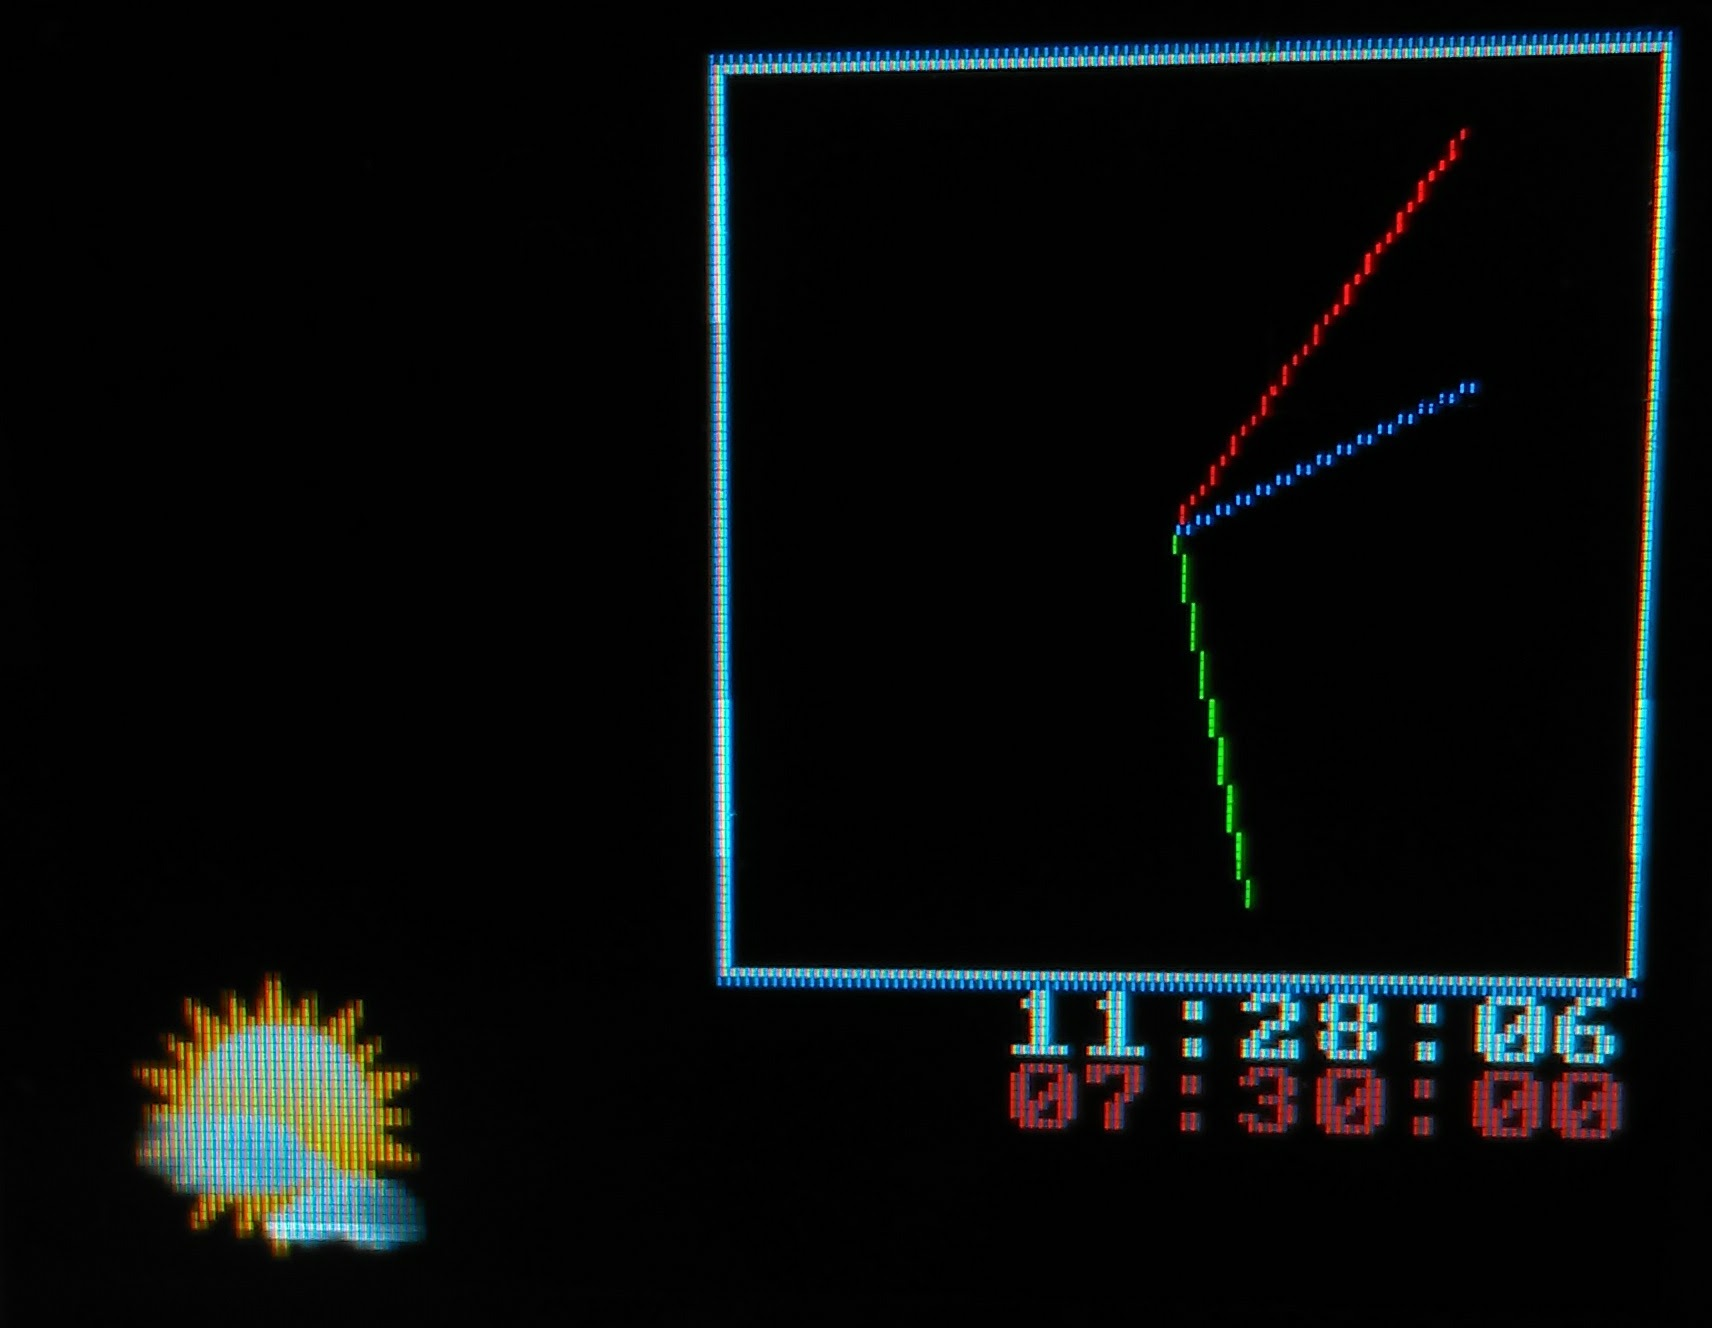
\includegraphics[width=0.4\textwidth]{./fig/clock_weather.png}
	\caption{Displaying basic functionality}
\end{figure}
\section{Software Server}
To obtain the most recent time, weather and email, a server back-end has been made. This server back-end is accessible trough a RESTful interface. An application can fire post requests with protobuf messages in the body. This will be decoded on the server and the right response will be given. The server backend is written in Java, and hosted on a Platform as a Service (Heroku \cite{other:heroku}). To accelerate RESTful java interface development, the spark framework has been chosen to develop with Spark \cite{other:spark}. Right now the server takes care of time and timezones, weather and email. The time is obtained based on location. The user will provide a city where the weather and time should be based on. This will be translated in a latitude and longitude trough Google api's. Google also provides a possibility to return a timezone based on latitude and longitude. The current time is requested from the server and translated with the timezone. Next is the weather, which is requested trough openweathermap \cite{other:weathermaps}. This is done once every 30 minutes, whereas the time is updated once every hour. The email functionality is provided trough javax mail \cite{other:javax}. A pitfall here is the use of security, that is something which has to be looked into in a future edition.
\begin{figure}[H]
	\centering
	\label{fig:block_server}
	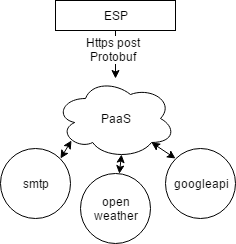
\includegraphics[width=0.4\textwidth]{fig/block_server.png}
	\caption{The system structure and hierarchy}
\end{figure}
Above in fig. \ref{fig:block_server} a rough sketch of the dataflow is shown
\section{Software ESP}
\label{sec:esp}
The ESP also had to be programmed, this is done in C++ as that is the most efficient and most supported framework available right now. The ESP relays all the protobuf messages from the xmega to the server backend. Right now this is done via http post requests. This can be optimized by the usage of websockets. However these were not functional yet during the time of development. This could enable ssl encryption to make it safer for sending sensitive data, and a more real time stream could be set up. Although the ESP is programmed in C++, a C version of protobuf has been used. This way it was possible to reuse the code already written for the xmega. A website also has been developed. This way the user can connect to the access point and set up the alarm, city, wifi connection and information shown. The website was created using html, css, javascript, bootstrap and jquerry. All made responsive for both phone and computer accessibility.
